%\documentclass{article}
\documentclass[12pt, letterpaper, onecolumn]{article}
\usepackage[top=1.0in, bottom=1.0in, left=1.0in, right=1.0in]{geometry} %onecolumn

\usepackage[pdftex, colorlinks=true, filecolor=blue, urlcolor=blue]{hyperref}
\usepackage{amsmath,amsthm,amssymb}
\usepackage{graphicx}

\newcommand{\projname}{p5}
\newcommand{\projnum}{5}

%\input{common}
\newenvironment{packed_item}{
\begin{itemize}
  \setlength{\itemsep}{1pt}
  \setlength{\parskip}{0pt}
  \setlength{\parsep}{0pt}
}{\end{itemize}}

\begin{document}

\title{Formulating LCP for Articulated Rigid Bodies}
\author{}
% Jie did the derivation, so kasiu feels bad about being the author :(
\date{}
%\date{Last Edited: Spring 2012}

\maketitle
\section{Overview}
The following document describes the construction of the matrices responsible for solving LCP (linear-complimentarity problems) for articulated rigid bodies in generalized coordinates. The document assumes familiarity with the mathematical construction of LCP. This was originally intended as a guide for the implementation of the LCP solver for the DART dynamics library.
\section{The Equations of Motion}
<<<<<<< HEAD
We begin our derivation from the following form of the equations of motion:
\begin{equation}
\label{eq:motionequations}
M\ddot{q} + C\dot{q} + kq = \tau + J^T{f_n}\vec{N} + J^TD\vec{f_d}
=======
We begin our derivation from the following form of the equations of
motion for an articulated rigid body system with one contact point:
\begin{equation}
\label{eq:motionequations}
M(\vc{q})\ddot{\vc{q}} + C(\vc{q}, \dot{\vc{q}}) = \tau + J^T f_n \vc{n} + J^T
D \vc{f}_d
>>>>>>> karen
\end{equation}
\\
The terms of this equation are as follows:
\begin{packed_item}
<<<<<<< HEAD
\item $kq$ is a term for elastic forces (used in problems such as FEM, but can be omitted for articulated bodies)
\item $\tau$ is the vector of external forces
\item $J$ is the Jacobian from Cartesian to generalized coordinates (with respect to forces)
\item $f_n$ is the magnitudes of the normal forces
\item $\vec{N}$ is the normal direction
\item $D$ is the discretized friction cone bases
\item $\vec{f_d}$ is a vector of forces along the discretized friction cone bases
\end{packed_item}
We can manipulate Equation \ref{eq:motionequations} as follows:
\begin{equation}
\label{eq:changemotionequations0}
M\ddot{q} = M\frac{(\dot{q}^{n+1}-\dot{q}^n)}{\Delta{t}}
\end{equation}
\begin{equation}
\label{eq:changemotionequations1}
M\frac{(\dot{q}^{n+1}-\dot{q}^n)}{\Delta{t}} = -C\dot{q}^n - kq^n + \tau^n + J^Tf_n\vec{N} + J^TD\vec{f_d} 
\end{equation}
\begin{equation}
\label{eq:changemotionequations2}
M\dot{q}^{n+1} = M\dot{q}^n - \Delta{t}(C\dot{q}^n + kq^n - \tau^n) + \Delta{t}(J^Tf_n\vec{N} + J^TD\vec{f_d})
\end{equation}
The first two terms on the right are known values. 
We group these into a single term $\tau^*$:
\begin{equation}
\label{eq:taustar}
\tau^* = M\dot{q}^n - \Delta{t}(C\dot{q}^n + kq^n - \tau^n)
=======
\item $\vc{q}$: the state vector
\item $M$: the mass matrix
\item $C$: Coriolis, centrifugal, and gravitational forces
\item $\tau$: internal generalized forces
\item $J$: the Jacobian matrix evaluated at the contact point
\item $\vc{n}$: the normal force direction (Figure \ref{fig:example}(a))
\item $f_n$: the magnitude of the normal force
\item $D$: discretized friction cone bases (Figure \ref{fig:example}(a))
\item $\vc{f}_d$: the magnitudes of tangent forces along the discretized friction cone bases
\end{packed_item}

\begin{figure}
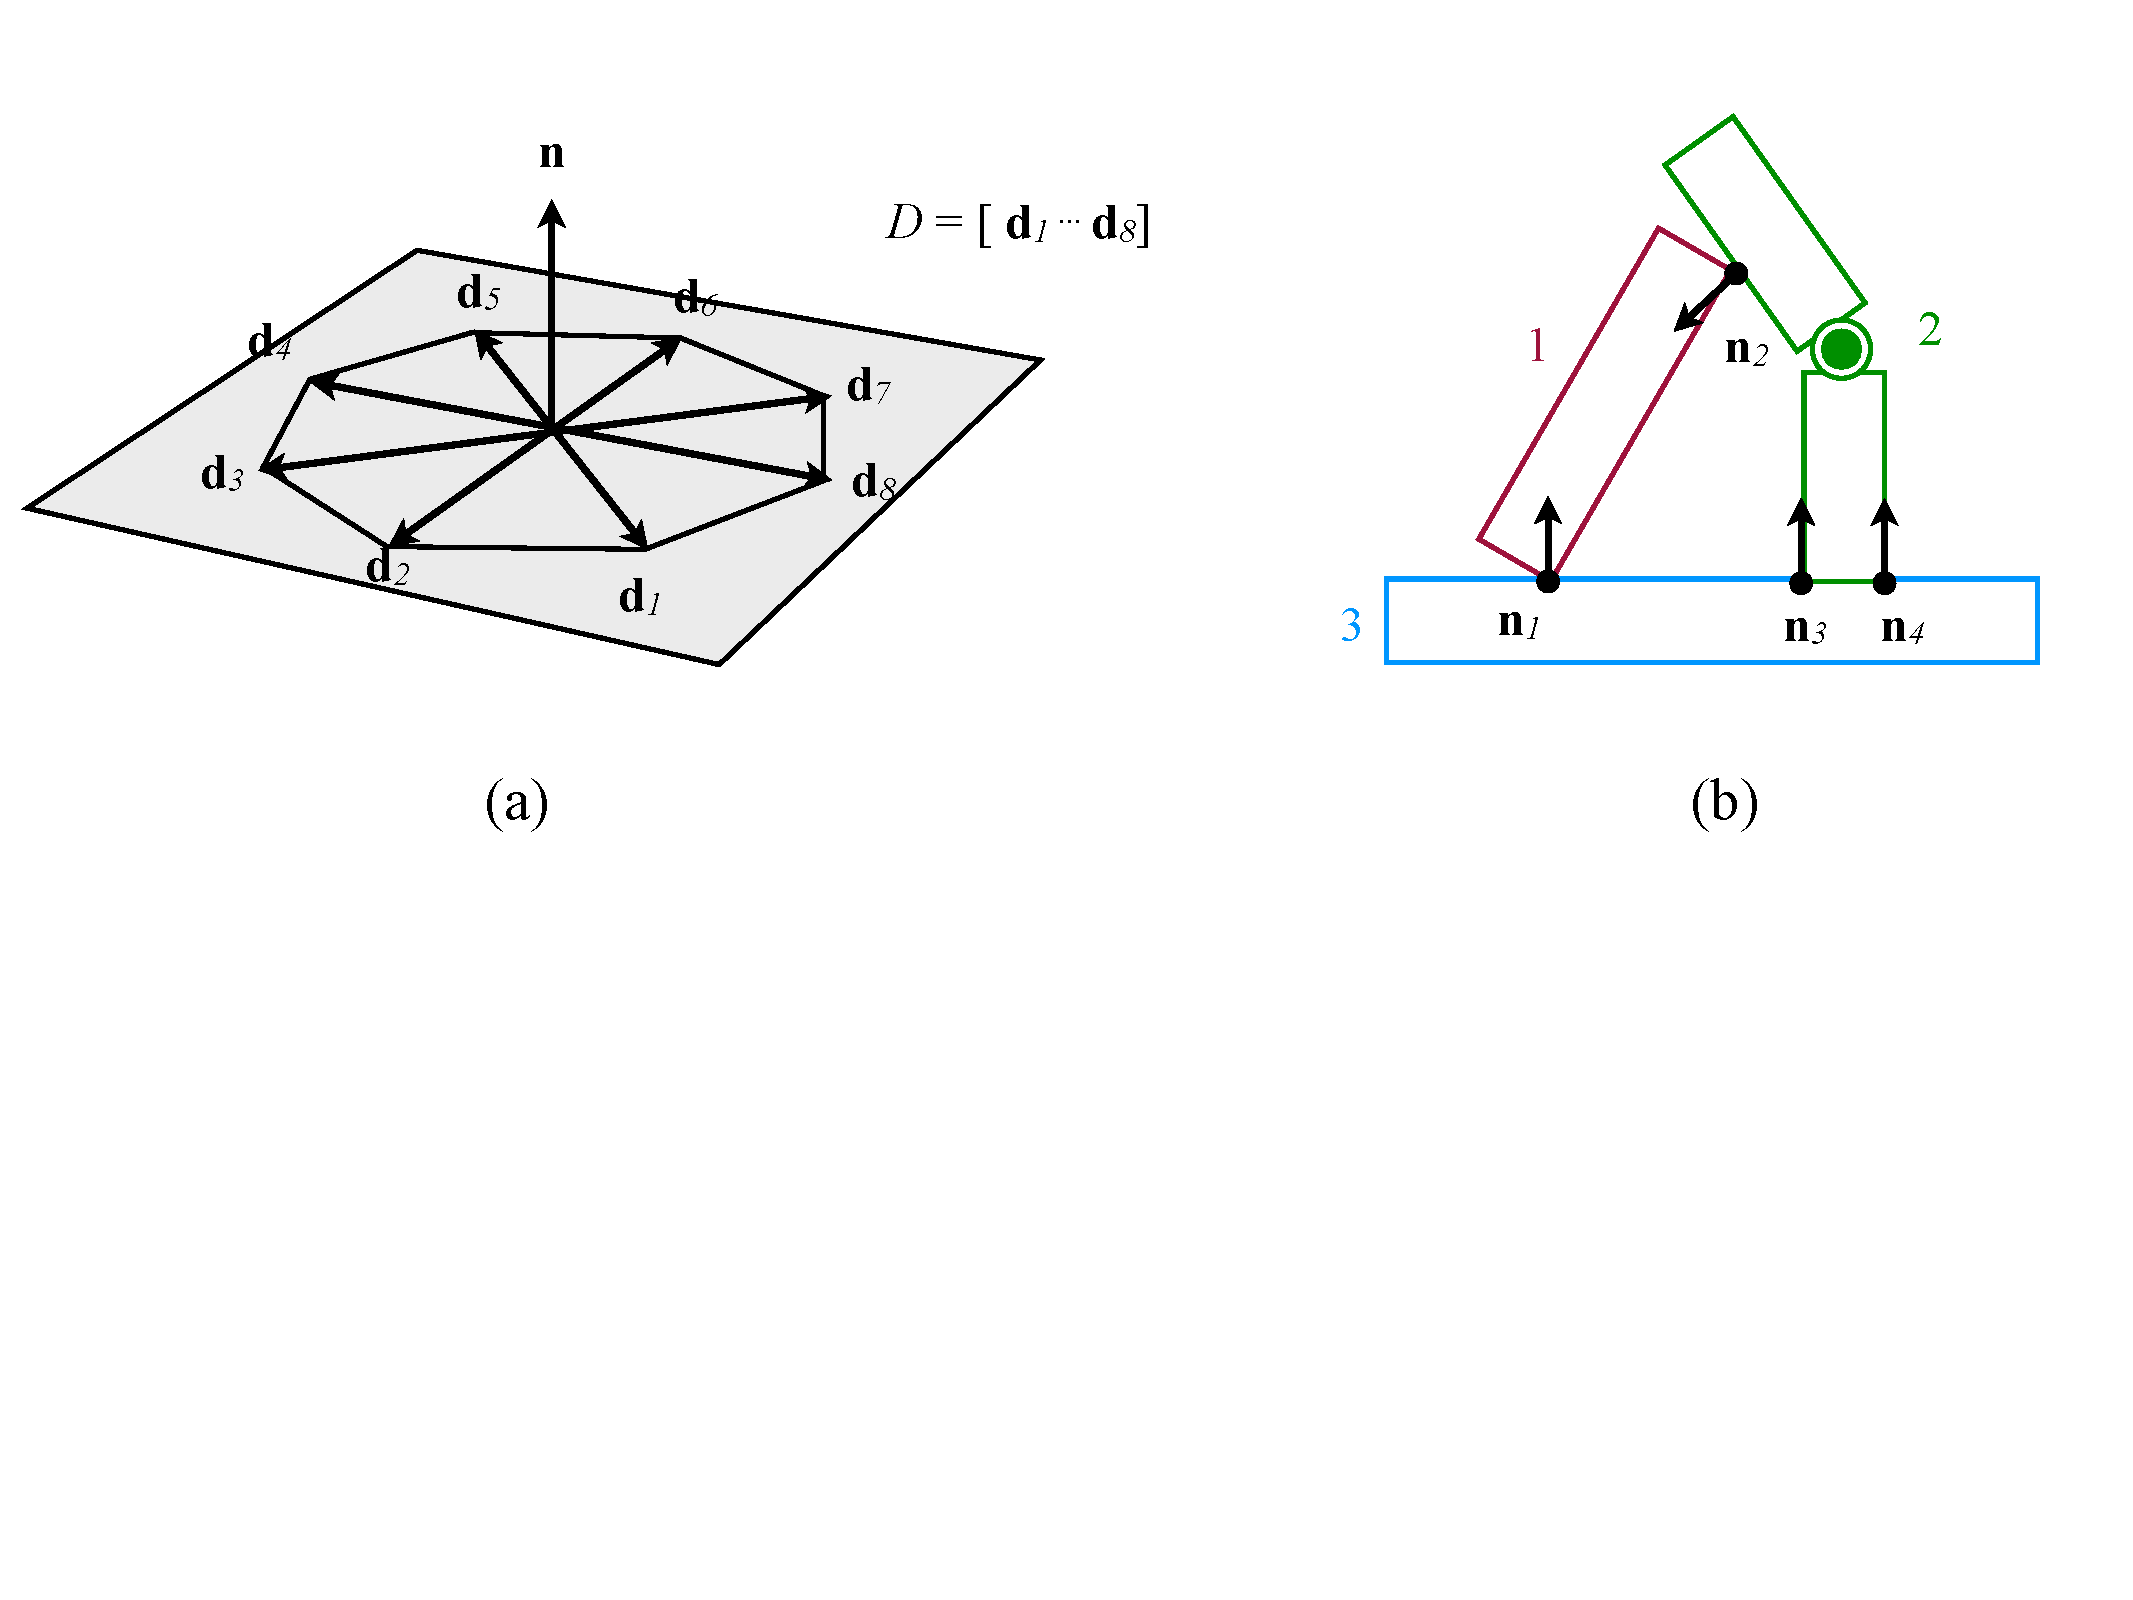
\includegraphics[width=6in]{example1.pdf}
\caption{An articulated system.}
\label{fig:example}
\end{figure}

We can discretize Equation \ref{eq:motionequations} as follows:
\begin{equation}
\label{eq:changemotionequations0}
M\ddot{\vc{q}} = M\frac{(\dot{\vc{q}}^{n+1}-\dot{\vc{q}}^n)}{\Delta{t}}
\end{equation}
\begin{equation}
\label{eq:changemotionequations1}
M\frac{(\dot{\vc{q}}^{n+1}-\dot{\vc{q}}^n)}{\Delta{t}} = -C(\vc{q}^n, \dot{\vc{q}}^n) + \tau^n + J^Tf_n\vc{n} + J^TD\vc{f}_d 
\end{equation}
\begin{equation}
\label{eq:changemotionequations2}
M\dot{\vc{q}}^{n+1} = M\dot{\vc{q}}^n - \Delta{t}(C(\vc{q}^n, \dot{\vc{q}}^n) - \tau^n) + \Delta{t}(J^Tf_n\vc{n} + J^TD\vc{f}_d)
\end{equation}
where superscripts $n$ and $n+1$ indicate the current and the next time
steps. In Equation \ref{eq:changemotionequations2} , the first two terms on the right are known values. 
We group these into a single term $\tau^*$:
\begin{equation}
\label{eq:taustar}
\tau^* = M\dot{\vc{q}}^n - \Delta{t}(C - \tau^n)
>>>>>>> karen
\end{equation}
We are then left with:
\begin{equation}
\label{eq:changemotionequations3}
<<<<<<< HEAD
M\dot{q}^{n+1} = \tau^* + \Delta{t}(J^Tf_n\vec{N} + J^TD\vec{f_d})
\end{equation}
At each time step, let $m$ denote the number of bodies in the system and $c$ denote the number of contact points.
For simplicity, we will ignore the timestep superscripts ($n$) of the generalized coordinates $q$ and its derivatives.
=======
M\dot{\vc{q}} = \tau^* + \Delta{t}(J^Tf_n\vc{n} + J^TD\vc{f}_d)
\end{equation}
where the unknown variables are the velocity of the state at the next time
step ($\dot{\vc{q}}$, superscript $n+1$ omitted for simplicity), the magnitude
of normal force ($f_n$), and the magnitudes of tangent forces ($\vc{f}_d$). 

Now let us consider the equations of motion for a more complex
situation shown in Figure \ref{fig:example}(b). There are four contact
points and three systems involved in the scene. We can stack the
equations of motion for each system in the following matrix form:

\begin{eqnarray}
\label{eq:changemotionequations4}
\left[\begin{matrix}M_1  & 0 & 0 \\ 0 & M_2 & 0 \\ 0 & 0 &
    M_3\end{matrix}\right]\left[\begin{matrix}\dot{q_1} \\ \dot{q_2}
    \\ \dot{q_3}\end{matrix}\right] = \left[\begin{matrix}{\tau_1}^*
    \\ {\tau_2}^* \\ {\tau_3}^*\end{matrix}\right] +
\Delta{t}\left[\begin{matrix}{J_{11}}^T\vc{n}_1 &
    {J_{12}}^T\vc{n}_2 & 0 & 0 \\ 0 & -J_{22}^T\vc{n}_2 & J_{23}^T
    \vc{n}_3 & J_{24}^T \vc{n}_4 \\ -J_{31}^T \vc{n}_1 & 0 & -J_{33}^T
    \vc{n}_3 & -J_{34}^T
    \vc{n}_4 \end{matrix}\right]\left[\begin{matrix}f_{n1} \\ f_{n2}
    \\ f_{n3} \\ f_{n4} \end{matrix}\right] \nonumber \\ +
\Delta{t}\left[\begin{matrix}J_{11}^T D_1 &
    J_{12}^TD_2 & 0 & 0 \\ 0 & -J_{22}^TD_2 & J_{23}^T
    D_3 & J_{24}^T D_4 \\ -J_{31}^T D_1 & 0 & -J_{33}^T
    D_3 & -J_{34}^T
    D_4 \end{matrix}\right]\left[\begin{matrix}\vc{f}_{d1} \\ \vc{f}_{d2} \\
    \vc{f}_{d3} \\ \vc{f}_{d4}\end{matrix}\right]
\end{eqnarray}
The subscript $i$ for $M_i$, $\dot{\vc{q}}_i$, and $\tau^*_i$ indicates the
$i$-th system, while the subscript $j$ for $\vc{n}_j$, $D_j$, $f_{nj}$,
and $\vc{f}_{dj}$ indicates the $j$-th contact. A Jacobian matrix
$J_{ij}$ has two subscripts indicating the Jacobian evaluated at
contact $j$ for the system $i$. 

For simplicity, we will rewrite some of these terms as matrices $N$ and $B$ as follows:
\begin{equation}
\label{eq:nbmatrix}
\begin{array}{cc}
N = \left[\begin{matrix}{J_{11}}^T\vc{n}_1 &
    {J_{12}}^T\vc{n}_2 & 0 & 0 \\ 0 & -J_{22}^T\vc{n}_2 & J_{23}^T
    \vc{n}_3 & J_{24}^T \vc{n}_4 \\ -J_{31}^T \vc{n}_1 & 0 & -J_{33}^T
    \vc{n}_3 & -J_{34}^T
    \vc{n}_4  \end{matrix}\right] \\
B = \left[\begin{matrix}J_{11}^T D_1 &
    J_{12}^TD_2 & 0 & 0 \\ 0 & -J_{22}^TD_2 & J_{23}^T
    D_3 & J_{24}^T D_4 \\ -J_{31}^T D_1 & 0 & -J_{33}^T
    D_3 & -J_{34}^T
    D_4 \end{matrix}\right]
\end{array}
\end{equation}
Assuming the total number of degrees of freedom for three systems is
$m$, the number of the contacts is $p$ ($p=4$ in Figure
\ref{fig:example}(b)), and the number of friction cone bases is $d$
($d = 8$ in Figure \ref{fig:example}(a)), the dimensions of $N$ and
$B$ are $m \times p$ and $m \times pd$, respectively. With these
substitutions, Equation \ref{eq:changemotionequations4} reduces to the
following:
\begin{equation}
\label{eq:changemotionequations5}
M\dot{\vc{q}} = \tau^* + \Delta{t} (N\vc{f}_n + B\vc{f}_d)
\end{equation}


\ignorethis{
At each time step, let $m$ denote the number of bodies in the system and $p$ denote the number of contact points.
For simplicity, we will ignore the time step superscripts ($n$) of the generalized coordinates $q$ and its derivatives.
>>>>>>> karen
\\
\\
Additionally, we use the notation $X_{ij}$ to describe a variable $X$, which corresponds to information about a contact between bodies $i$ and $j$.
For example, we would denote the normal $\vec{N}$ at the contact point between $i$ and $j$ as $\vec{N_{ij}}$.
\\
\\
We illustrate the following derivation using an example environment consisting of $(m = 3)$ rigid bodies in contact at $(c = 2)$ points. Without loss of generality, assume bodies 1 and 2 are in contact, and bodies 2 and 3 are in contact.
\\
\\
Using this example, we can rewrite Equation \ref{eq:changemotionequations3} as follows:
\begin{equation}
\label{eq:changemotionequations4}
\left[\begin{matrix}M_1  & 0 & 0 \\ 0 & M_2 & 0 \\ 0 & 0 & M_3\end{matrix}\right]\left[\begin{matrix}\dot{q_1} \\ \dot{q_2} \\ \dot{q_3}\end{matrix}\right] = \left[\begin{matrix}{\tau_1}^* \\ {\tau_2}^* \\ {\tau_3}^*\end{matrix}\right] + \Delta{t}\left[\begin{matrix}{J_{21}}^T\vec{N_{21}} & 0 \\ {J_{12}}^T\vec{N_{12}} & {J_{32}}^T\vec{N_{32}} \\ 0 & {J_{23}}^T\vec{N_{23}} \end{matrix}\right]\left[\begin{matrix}f_{n1} \\ f_{n2}\end{matrix}\right] + \Delta{t}\left[\begin{matrix}{J_{21}}^TD_{21} & 0 \\ {J_{12}}^TD_{12} & {J_{32}}^TD_{32} \\ 0 & {J_{23}}^TD_{23} \end{matrix}\right]\left[\begin{matrix}f_{d1} \\ f_{d2}\end{matrix}\right]
\end{equation}
For simplicity, we'll rewrite some of these terms as variables $N$ and $B$ as follows:
\begin{equation}
\label{eq:nbmatrix}
\begin{array}{cc}
N = \Delta{t}\left[\begin{matrix}{J_{21}}^T\vec{N_{21}} & 0 \\ {J_{12}}^T\vec{N_{12}} & {J_{32}}^T\vec{N_{32}} \\ 0 & {J_{23}}^T\vec{N_{23}} \end{matrix}\right] \\
B = \Delta{t}\left[\begin{matrix}{J_{21}}^TD_{21} & 0 \\ {J_{12}}^TD_{12} & {J_{32}}^TD_{32} \\ 0 & {J_{23}}^TD_{23} \end{matrix}\right]
\end{array}
\end{equation}
Note here that $N$ is a matrix, not to be confused with $N_{ij}$, which is a vector.
\\
\\
Also, we note that $N$ is a $(m^* \times c)$ matrix, instead of a full $(m^* \times 2c)$ matrix (as each contact corresponds to two normal vectors). This exploits the fact that $\vec{N_{ij}} = -\vec{N_{ij}}$ and that the magnitude of these vectors (forces) are the same. Thus, we can condense the matrix. Similarly, $B$ takes advantage of this as well. Here $m^*$ depends on both $m$, as well as the DOFs of each $q_i$. ($m^*$ is the product of $m$ and the respective number of DOFs for each $q_i$.)
\\
\\
<<<<<<< HEAD
=======

>>>>>>> karen
With these substitutions, Equation \ref{eq:changemotionequations4} reduces to the following:
\begin{equation}
\label{eq:changemotionequations5}
M\dot{q} = \tau^* + N\vec{f_n} + B\vec{f_d}
<<<<<<< HEAD
\end{equation}
=======
\end{equation}
}
>>>>>>> karen

\section{LCP Formulation}
Recall that we need $V_n$ (the relative velocity), which is given by the following expression:
\begin{equation}
\label{eq:vn0}
V_n = N^T\dot{q}
\end{equation}
Expanding this out using the example problem yields the following:
\begin{equation}
\label{eq:vn1}
V_n = \left[\begin{matrix}\vec{N_{21}}^TJ_{21} & \vec{N_{12}}^TJ_{12} & 0 \\ 0 & \vec{N_{32}}^TJ_{32} & \vec{N_{23}}^TJ_{23}\end{matrix}\right]\left[\begin{matrix}\dot{q_1} \\ \dot{q_2} \\ \dot{q_3}\end{matrix}\right]
\end{equation}
\begin{equation}
\label{eq:vn2}
V_n = \left[\begin{matrix}\vec{N_{21}}^TJ_{21}\dot{q_1} + \vec{N_{12}}^TJ_{12}\dot{q_2} \\ \vec{N_{32}}^TJ_{32}\dot{q_2} + \vec{N_{23}}^TJ_{23}\dot{q_3}\end{matrix}\right]
\end{equation}
Since $\vec{N_{ij}} = -\vec{N_{ji}}$, we can reduce this further:
\begin{equation}
\label{eq:vn3}
V_n = \left[\begin{matrix}\vec{N_{21}}^T(J_{21}\dot{q_1} - J_{12}\dot{q_2}) \\ \vec{N_{32}}^T(J_{32}\dot{q_2} - J_{23}\dot{q_3})\end{matrix}\right]
\end{equation}

\subsection{Normal Direction Constraints}
We now begin revisiting the constraints for LCP.
\begin{packed_item}
\item $\vec{f_n} \geq 0$
\item $\vec{v_n} \geq 0$
\item $\vec{v_n}^T\vec{f_n} = 0$
\end{packed_item}
The first expression ensures there is no pulling force. The second expression prevents penetration with the contact surface. The third expression constrains the normal force based on the velocity. If $\vec{v_n} > 0$, then $\vec{f_n} = 0$ (in takeoff). If $\vec{v_n} = 0$, then $\vec{f_n} \geq 0$ (in contact).

\subsection{Friction Cone Constraints}
\begin{packed_item}
\item $\vec{\lambda} \geq 0$
\item $\mu\vec{f_n} - E^T\vec{f_d} \geq 0$
\item $\lambda(\mu\vec{f_n} - E^T\vec{f_d}) = 0$
% Should this be \vec{lamba}?
\end{packed_item}
Here $E$ is a $(cd \times c)$ matrix where $d$ is the number of contact (friction cone) directions and $c$ is the number of contacts (as defined above). As an example, the structure of $E$ for a problem with $(d = 3)$ contact directions and $(c = 2)$ contacts would be as follows:
\begin{equation}
\label{eq:ematrix}
E = \left[\begin{matrix}1 & 0 \\ 1 & 0 \\ 1 & 0 \\ 0 & 1 \\ 0 & 1 \\ 0 & 1\end{matrix}\right]
\end{equation}
Additionally, $\vec{\lambda}$ is a vector of length $c$ that contains all of the $\lambda$ values.
\begin{equation}
\label{eq:lambda}
\vec{\lambda} = \left[\begin{matrix}\lambda_1 \\ \lambda_2 \\ .. \\ \lambda_c\end{matrix}\right]
\end{equation}

\subsection{Directional Friction Constraints}
\begin{packed_item}
\item $\vec{f_d} \geq 0$
\item $B^T\dot{q} - E\vec{\lambda} \geq 0$
\item $(B^T\dot{q} - E\vec{\lambda})^T\vec{f_d} = 0$
\end{packed_item}
From this, we can construct the following linear system of equations:
\begin{equation}
\label{eq:bigsystem}
\begin{array}{cc}
\left[\begin{matrix}0 \\ a \\ b \\ c \end{matrix}\right] = \left[\begin{matrix}M & -N & -B & 0 \\ N^T & 0 & 0 & 0 \\ B^T & 0 & 0 & E \\ 0 & \mu & -E^T & 0\end{matrix}\right]\left[\begin{matrix}\vec{\dot{q}} \\ \vec{f_n} \\ \vec{f_d} \\ \vec{\lambda}\end{matrix}\right] + \left[\begin{matrix}-\tau^* \\ 0 \\ 0 \\0\end{matrix}\right] \\
\begin{matrix}
\left[\begin{matrix}\vec{f_n} \\ \vec{f_d} \\ \vec{\lambda}\end{matrix}\right] \geq 0, & 
\left[\begin{matrix}a \\ b \\ c\end{matrix}\right] \geq 0, &
\left[\begin{matrix}a \\ b \\ c\end{matrix}\right]^T\left[\begin{matrix}\vec{f_n} \\ \vec{f_d} \\ \vec{\lambda}\end{matrix}\right] = 0
\end{matrix}
\end{array}
\end{equation}
The first row of the system is based on Equation \ref{eq:changemotionequations5}. The remaining three rows, as well as the constraints, encapsulate the nine LCP conditions described above.
\\
\\
Here $(a, b, c)$ are the results of the following constraints: 
\begin{packed_item}
\item $\vec{v_n} \geq 0$
\item $\mu\vec{f_n} - E^T\vec{f_d} \geq 0$
\item $B^T\dot{q} - E\vec{\lambda} \geq 0$
\end{packed_item}
The expression for $\vec{v_n}$ comes from solving for the relative velocity in Equation \ref{eq:vn3}.
\\
\\
Unfortunately, the construction described is in MLCP (Mixed LCP) form. To convert it to standard form, we need to make a few adjustments.
\section{Standard LCP Form}
Standard LCP is of the following form:
\begin{equation}
\begin{array}{cc}
\vec{w} = A\vec{z} + \vec{q} \\
\vec{w} \geq 0 \\
\vec{z} \geq 0 \\
\vec{w}^T\vec{z} = 0
\end{array}
\end{equation}
If we solve for $\dot{q}$, we get:
\begin{equation}
\dot{q} = M^{-1}(V\vec{f_n} + B\vec{f_d} + \tau^*)
\end{equation}
We can then reorder Equation \ref{eq:bigsystem} slightly to get the following:
\begin{equation}
\label{eq:slcp0}
\left[\begin{matrix}a \\ b \\ c\end{matrix}\right] = \left[\begin{matrix}N^TM^{-1}N & N^TM^{-1}B & 0 \\ B^TM^{-1}N & B^TM^{-1}B & E \\ \mu & -E^T & 0\end{matrix}\right]\left[\begin{matrix}\vec{f_n} \\ \vec{f_d} \\ \vec{\lambda}\end{matrix}\right] + \left[\begin{matrix}N^TM^{-1}\tau^* \\ B^TM^{-1}\tau^* \\ 0\end{matrix}\right]
\end{equation}
Where:
\begin{equation}
\label{eq:slcp1}
\begin{array}{cc}
\vec{w} = \left[\begin{matrix}a \\ b \\ c\end{matrix}\right] \\
A = \left[\begin{matrix}N^TM^{-1}N & N^TM^{-1}B & 0 \\ B^TM^{-1}N & B^TM^{-1}B & E \\ \mu & -E^T & 0\end{matrix}\right] \\
\vec{z} = \left[\begin{matrix}\vec{f_n} \\ \vec{f_d} \\ \vec{\lambda}\end{matrix}\right] \\
\vec{q} = \left[\begin{matrix}N^TM^{-1}\tau^* \\ B^TM^{-1}\tau^* \\ 0\end{matrix}\right]
\end{array}
\end{equation}
Once we have $\vec{w}$ and $\vec{z}$, we can plug values back into the equations of motion to get $\dot{q}^{n + 1}$.
\end{document}